\documentclass[11pt]{article}
\usepackage[margin=1in]{geometry}
\usepackage{amsmath,amssymb,amsthm}
\usepackage{lmodern}
\usepackage[T1]{fontenc}
\usepackage{microtype,xcolor,framed,graphicx,float,listings}
\usepackage[colorlinks=true,linkcolor=blue!60!black]{hyperref}

\definecolor{shadecolor}{RGB}{240,244,250}
\newcommand{\R}{\mathbb{R}}
\newcommand{\T}{^{\mathsf T}}
\newcommand{\ones}{\mathbf{1}}
\newcommand{\answer}[1]{\begin{shaded}\noindent\textbf{Answer.} #1\end{shaded}}
\lstset{language=Python,basicstyle=\ttfamily\scriptsize,
  keywordstyle=\color{blue!60!black},commentstyle=\color{black!55},
  frame=single,rulecolor=\color{black!20},breaklines=true,
  showstringspaces=false,columns=fullflexible}
\setlength{\parindent}{0pt}
\setlength{\parskip}{0.5em}

\begin{document}
\begin{center}
{\Large\bfseries Optimization --- Homework 3}\\[4pt]
{\large Solutions}\\[6pt]
Mitchel Carson \hfill September 19, 2026
\end{center}
\medskip

\textit{Notation.} Vector inequalities are componentwise. $A_j$ denotes column $j$ of $A$, and $a_i\T$ denotes row $i$.

\section*{Problem 1. Computing the dual}
The primal is
\[
\begin{aligned}
\min\quad &x_1-x_2\\
\text{s.t.}\quad &2x_1+3x_2-x_3+x_4\le0,\\
&3x_1+x_2+4x_3-2x_4\ge3,\\
&-x_1-x_2+2x_3+x_4=6,\\
&x_1\le0,\quad x_2,x_3\ge0,\quad x_4\text{ free}.
\end{aligned}
\]
Let $A$ be the matrix of the three general constraints, $b=(0,3,6)\T$, and $c=(1,-1,0,0)\T$. Using the Lagrangian
\[
L(x,p)=c\T x+p\T(b-Ax),
\]
choose $p_1\le0$, $p_2\ge0$, and $p_3$ free, so that $L(x,p)\le c\T x$ for every primal-feasible $x$.

The dual function is
\[
g(p)=p\T b+
\inf_{x_1\le0,\;x_2,x_3\ge0,\;x_4\in\R}
\sum_{j=1}^4(c_j-p\T A_j)x_j.
\]
This infimum is finite precisely when
\[
c_1-p\T A_1\le0,\qquad
c_2-p\T A_2\ge0,\qquad
c_3-p\T A_3\ge0,\qquad
c_4-p\T A_4=0.
\]
Under these conditions the infimum is $0$, attained at $x=0$; otherwise it is $-\infty$. Thus maximising $g(p)$ gives
\answer{
\[
\begin{aligned}
\max\quad &3p_2+6p_3\\
\text{s.t.}\quad &2p_1+3p_2-p_3\ge1,\\
&3p_1+p_2-p_3\le-1,\\
&-p_1+4p_2+2p_3\le0,\\
&p_1-2p_2+p_3=0,\\
&p_1\le0,\quad p_2\ge0,\quad p_3\text{ free}.
\end{aligned}
\]
}

\newpage
\section*{Problem 2. A theorem of the alternative}
For $A\in\R^{m\times n}$, prove the equivalence of:
\begin{enumerate}
\item[(i)] $Ax\ge0$ and $x\ge0$ imply $x_1=0$;
\item[(ii)] there exists $p\ge0$ such that $p\T A\le0$ and $p\T A_1<0$.
\end{enumerate}

\begin{proof}[Proof of (ii) $\Rightarrow$ (i)]
Let $p$ satisfy (ii), and suppose $Ax\ge0$ and $x\ge0$. Then
\[
0\le p\T Ax
=\sum_{j=1}^n(p\T A_j)x_j
\le(p\T A_1)x_1
\le0.
\]
The first inequality uses $p\ge0$ and $Ax\ge0$; the remaining inequalities use $p\T A_j\le0$ and $x_j\ge0$. Consequently $(p\T A_1)x_1=0$. Since $p\T A_1<0$, we obtain $x_1=0$.
\end{proof}

\begin{proof}[Proof of (i) $\Rightarrow$ (ii)]
Consider the primal--dual pair
\[
\begin{aligned}
\text{(P)}\quad &\min_{x\ge0}\ -x_1
&&\text{s.t. }Ax\ge0,\\[5pt]
\text{(D)}\quad &\max_{p\ge0}\ 0
&&\text{s.t. }A\T p\le-e_1,
\end{aligned}
\]
where $e_1=(1,0,\ldots,0)\T\in\R^n$. The dual constraints follow from the primal objective coefficient $-e_1$, the nonnegative variables $x$, and the zero right-hand side.

The primal is feasible at $x=0$. By (i), every feasible $x$ has $x_1=0$, so its optimal value is $0$ and is attained. Strong LP duality therefore guarantees a feasible dual solution $p$. It satisfies
\[
p\ge0,\qquad p\T A_1\le-1<0,\qquad
p\T A_j\le0\quad(j=2,\ldots,n),
\]
which proves (ii).
\end{proof}

\newpage
\section*{Problem 3. A small infeasible subsystem}
Let $A\in\R^{500\times100}$ and suppose $Ax\le b$ is infeasible. We prove that at most $101$ of its inequalities already form an infeasible system.

\paragraph{1. Introduce a common violation variable.}
Consider
\[
\text{(P)}\qquad
\min_{x\in\R^{100},\;t\in\R}\ t
\quad\text{s.t.}\quad a_i\T x-t\le b_i,
\quad i=1,\ldots,500.
\]
This LP is feasible: set $x=0$ and take $t$ sufficiently large. Every feasible pair has $t>0$, since $t\le0$ would imply $Ax\le b$. Thus the objective is bounded below. A feasible LP with a finite lower bound attains its optimum, so there is an optimal pair $(x^\star,t^\star)$ with $t^\star>0$.

\paragraph{2. Choose an optimal dual solution with small support.}
Writing the constraints as $-a_i\T x+t\ge-b_i$ gives the dual
\[
\text{(D)}\qquad
\max_p\ -b\T p
\quad\text{s.t.}\quad A\T p=0,\quad
\ones\T p=1,\quad p\ge0,
\]
where $\ones\in\R^{500}$ is the all-ones vector. Strong duality gives an attained dual optimum equal to $t^\star$.

The dual feasible set is a nonempty compact polytope, since it is a closed subset of the simplex $\{p\ge0:\ones\T p=1\}$. A linear objective on this polytope has an optimal extreme point $p^\star$. At an extreme point of a standard-form polyhedron, the equality-matrix columns corresponding to positive variables are linearly independent. Here the equality matrix is
\[
\begin{pmatrix}A\T\\\ones\T\end{pmatrix}
\in\R^{101\times500}.
\]
Therefore the support $S=\{i:p_i^\star>0\}$ satisfies $|S|\le101$.

\paragraph{3. Prove that the inequalities in $S$ are infeasible.}
Complementary slackness for $(x^\star,t^\star)$ and $p^\star$ gives
\[
p_i^\star\bigl(b_i-a_i\T x^\star+t^\star\bigr)=0.
\]
Hence $b_i=a_i\T x^\star-t^\star$ for $i\in S$, and the dual equalities yield
\[
\sum_{i\in S}p_i^\star b_i
=\left(\sum_{i\in S}p_i^\star a_i\right)\T x^\star
-t^\star\sum_{i\in S}p_i^\star
=-t^\star<0.
\]
If some $x$ satisfied $a_i\T x\le b_i$ for every $i\in S$, then
\[
0=\left(\sum_{i\in S}p_i^\star a_i\right)\T x
\le\sum_{i\in S}p_i^\star b_i
=-t^\star<0,
\]
a contradiction. Thus the subsystem indexed by $S$ is infeasible and contains at most $101$ inequalities. The remaining inequalities can be discarded while preserving infeasibility. Figure~\ref{fig:small-subsystem} illustrates the result in two dimensions.\hfill$\square$

\newpage
\section*{Illustration and code for Problem 3}
For $n=2$, the three inequalities $x_2\le0$, $x_2\ge x_1+1$, and $x_2\ge-x_1+1$ are jointly infeasible, although every pair is feasible. Thus the bound $n+1=3$ is attained in this example.

\begin{figure}[H]
\centering
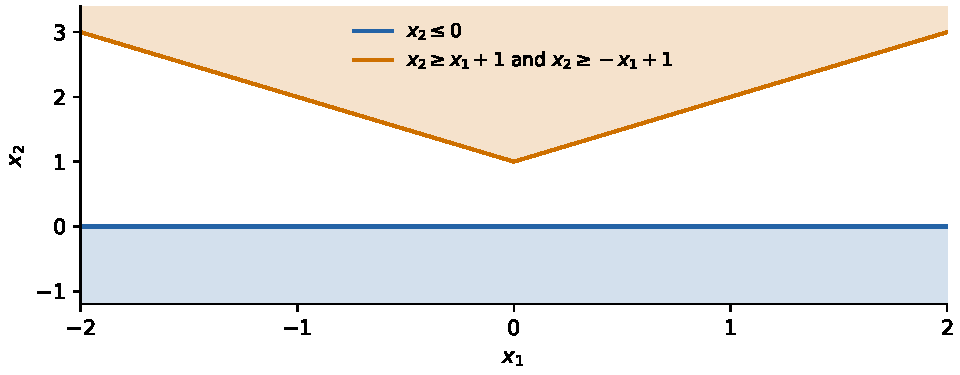
\includegraphics[width=.8\textwidth]{figures/p3_focused_example.pdf}
\caption{The blue half-plane and the orange intersection of the other two half-planes are disjoint. With rows ordered as above, $p=(2,1,1)\T$ satisfies $p\ge0$, $A\T p=0$, and $b\T p=-2<0$, certifying infeasibility.}
\label{fig:small-subsystem}
\end{figure}

The following Python code generates the figure and checks the certificate and pairwise feasibility using integer arithmetic. It illustrates the general proof above.
\lstinputlisting{focused_example.py}

\end{document}
